\chapter{Experiments and Results}\label{chp:results}

\section{Setting up the SLAM Algorithms}\label{sec:slam}

The following configuration was used for each of the tested algorithms. If not specified, the default configuration is being used. Cartographer is the only algorithm that also requires an external Lua file for configuration. All algorithms require the same hardware setup: a source of odometry, in this case a transformation from the robot fixed frame \texttt{odom\_combined} to \texttt{base\_link} and the laser scanner data, represented by the topic \texttt{scan\_unified}, that combines the data from all three lasers scanners on the robot base.

Every algorithm cycle then publishes the calculated map into the \texttt{/map} topic and a correction of odometry using a transformation from \texttt{map} to \texttt{odom\_combined}. This transformation is a small displacement between the two frames to account for errors in the odometry for the robot that accumulates over time and can be reduced by taking the pose corrected by SLAM.

\subsection{Gmapping}

To start Gmapping, we call the launch file shown in Listing~\ref{lst:gmapping}. It starts the node \texttt{slam\_gmapping} from package \texttt{gmapping}. The laser scan topic is remapped to match the robot topic name with the \texttt{remap} tag and the odometry frame is provided as \texttt{odom\_combined}. The \texttt{map\_update\_interval} and number of particles are kept in the default configuration. The \texttt{xmin}, \texttt{xmax}, \texttt{ymin} and \texttt{ymax} are the initial size of the resulting map in meters and won't impact the results, as they are automatically increased if the map needs to be bigger. The \texttt{delta} is the map resolution and is kept at the default value of 0.05 pixels/meter.

\begin{lstlisting}[caption={Gmapping launch file.},label={lst:gmapping},language=XML]
<launch>
  <node pkg="gmapping" type="slam_gmapping" name="slam_mapping" output="screen">
    <remap from="scan" to="scan_unified"/>
    <param name="odom_frame" type="string" value="odom_combined"/>
    <param name="map_update_interval" value="5.0"/>
    <param name="particles" value="30"/>
    <param name="xmin" value="-8"/>
    <param name="ymin" value="-8"/>
    <param name="xmax" value="8"/>
    <param name="ymax" value="8"/>
    <param name="delta" value="0.05"/> <!-- map_resolution -->
  </node>
</launch>
\end{lstlisting}

\subsection{Hector}

The Hector mapping node is started using the launch script in Listing~\ref{lst:hector}, starting the node \texttt{hector\_mapping} from package \texttt{hector\_mapping}. We first remap the laser scan to the right topic and use the adequate frame names for the map, base link and odometry link. The \texttt{pub\_map\_odom\_transform} is set to True to publish the transform from \texttt{map} to \texttt{odom\_combined}. The \texttt{laser\_min\_dist} is set to the minimum value registered for the COB laser scanners.

\begin{lstlisting}[caption={Hector launch file.},label={lst:hector},language=XML]
<launch>
  <node pkg="hector_mapping" type="hector_mapping" name="slam_mapping"    output="screen">
    <remap from="scan" to="scan_unified"/>
    <param name="map_frame" value="map" />
    <param name="base_frame" value="base_link" />
    <param name="odom_frame" value="odom_combined" />
    <param name="pub_map_odom_transform" value="true"/>
    <param name="laser_min_dist" value="0.05">
  </node>
</launch>
\end{lstlisting}

\subsection{Karto}

The Karto mapping node is started using the launch script in Listing~\ref{lst:karto}, starting the node \texttt{slam\_karto} from package \texttt{slam\_karto}. We only have to set the scan and odometry frames. The \texttt{map\_update\_interval} and \texttt{resolution} are set to the same values as Gmapping.

\begin{lstlisting}[caption={Karto launch file.},label={lst:karto},language=XML]
<launch>
  <node pkg="slam_karto" type="slam_karto" name="slam_mapping" output="screen">
    <remap from="scan" to="scan_unified"/>
    <param name="odom_frame" value="odom_combined"/>
    <param name="map_update_interval" value="5"/>
    <param name="resolution" value="0.05"/>
  </node>
</launch>
\end{lstlisting}

\subsection{Cartographer}

The Cartographer node requires a lot of configuration compared to the other SLAM algorithms. Two separate nodes have to be called at start, as seen in Listing~\ref{lst:cartographer}: the \texttt{cartographer\_node} and \texttt{cartographer\_occupancy\_grid\_node}, both from package \texttt{cartographer\_ros}.

The main Cartographer node does all the sub-map generation and takes as parameters a Lua file with the algorithm configuration, shown in Listing~\ref{lst:cartographer_lua}. The configuration file uses all the default parameters available in Cartographer example files (in file \texttt{backpack\_2d.lua}), with the exception that the IMU was disabled, as COB doesn't have one. The frames were set accordingly and the option \texttt{provide\_odom\_frame} was set to true to get the map to odometry transform during execution. The laser scan was changed from multi-echo laser scan to laser scan.

The second node is the occupancy grid node, that reads data from the sub-map list and republishes into the \texttt{/map} topic as a standard Occupancy Grid message from ROS. The resolution is also set to 0.05 pixels/meter.

\begin{lstlisting}[caption={Cartographer launch file.},label={lst:cartographer},language=XML]
<launch>
  <!-- Arguments -->
  <arg name="configuration_basename" default="cartographer.lua"/>

  <!-- cartographer_node -->
  <node pkg="cartographer_ros" type="cartographer_node" name="slam_mapping"
        args="-configuration_directory $(find cob_bringup_sim)/launch
              -configuration_basename $(arg configuration_basename)"
        output="screen">
    <remap from="scan" to="scan_unified" />
  </node>

  <!-- cartographer_occupancy_grid_node -->
  <node pkg="cartographer_ros" type="cartographer_occupancy_grid_node"
        name="cartographer_occupancy_grid_node"
        args="-resolution 0.05" />
</launch>
\end{lstlisting}

\begin{lstlisting}[caption={Cartographer Lua configuration.},label={lst:cartographer_lua},language=Python]
include "map_builder.lua"
include "trajectory_builder.lua"

options = {
  map_builder = MAP_BUILDER,
  trajectory_builder = TRAJECTORY_BUILDER,
  map_frame = "map",
  tracking_frame = "base_link",
  published_frame = "base_link",
  odom_frame = "odom_combined",
  provide_odom_frame = true,
  use_odometry = false,
  num_laser_scans = 1,
  num_multi_echo_laser_scans = 0,
  num_subdivisions_per_laser_scan = 10,
  num_point_clouds = 0,
  lookup_transform_timeout_sec = 0.2,
  submap_publish_period_sec = 0.3,
  pose_publish_period_sec = 5e-3,
  trajectory_publish_period_sec = 30e-3,
  rangefinder_sampling_ratio = 1.,
  odometry_sampling_ratio = 1.,
  imu_sampling_ratio = 1.,
}

MAP_BUILDER.use_trajectory_builder_2d = true
TRAJECTORY_BUILDER_2D.num_accumulated_range_data = 10
TRAJECTORY_BUILDER_2D.use_imu_data = false

return options
\end{lstlisting}

\section{Collecting data} \label{sec:collecting_data}

For data collection, we first start the robot using the command line. We are using \texttt{cob4-9} to avoid having to load unnecessary parts of the robot like the arms or the cameras.

\begin{verbatim}
roslaunch cob_bringup_sim robot.launch robot:=cob4-9 robot_env:=test1
\end{verbatim}

We then launch the controller to be able to drive the robot around using the keyboard.

\begin{verbatim}
roslaunch cob_teleop teleop_keyboard.launch 
\end{verbatim}

Finally, the data is recorded using the rosbag tool. We obviously need the \texttt{/tf}, \texttt{/tf\_static} and \texttt{/scan\_unified} for the SLAM algorithms. The \texttt{/base\_pose\_ground\_truth} is the ground truth data and will be later on used for comparison between algorithms. The \texttt{/base/twist\_controller/command} and  \texttt{/base/odometry\_controller/odometry} are respectively the commands given by the joystick and the calculated odometry after the command has been executed by the robot, and are recorded in case the bag files need to be re-executed.

\begin{verbatim}
rosbag record /base/odometry_controller/odometry
              /base/twist_controller/command
              /base_pose_ground_truth
              /scan_unified
              /tf
              /tf_static
\end{verbatim}

The data is recorded into a file that can be played at will and work as the real robot is sending the scans. This ensures every algorithm will get the same working data in the comparisons.

\section{Running the automated reconstruction}

All the steps required for data parsing by the SLAM algorithms were automated to ensure minimal human interaction is required. Once the data has been collected in the previous step, it can be played using the launch file shown in Listing~\ref{lst:parser}.

First, we set the parameters and arguments required. The \texttt{use\_sim\_time} ensures the clock will be used from the bag file, to avoid inconsistencies with time. The robot is set to \texttt{cob4-9} because this model will be uploaded for visualization purposes, and it's not required to run the SLAM. We then select the bag file and the algorithm to run together.

The launch file then calls the mapping algorithm, which will launch one of the files described on \prettyref{sec:slam}. Finally, we call the \texttt{rosbag play} node that will play back data already collected to the algorithm, providing clock with the option \texttt{--clock} and with a delay \texttt{-d 5} of 5 seconds to ensure all nodes are initialized before replaying data.

The last include calls for the RVIZ visualization if requested, as shown on \prettyref{fig:rviz_mapping}.

\begin{lstlisting}[caption={Automated data parser.},label={lst:parser},language=XML]
<launch>

  <!-- First set up sim time -->
  <param name="use_sim_time" value="true" />

  <!-- define arguments -->
  <arg name="robot" default="cob4-9"/>
  <arg name="bag" default="test1"/>
  <arg name="slam" default="gmapping"/>

  <!-- Call mapping -->
  <include file="$(find cob_bringup_sim)/launch/cob_$(arg slam).xml" />

  <!-- Play bag data with clock -->
  <node pkg="rosbag" type="play" name="player" output="screen" args="--clock -q -d 5 $(find cob_bringup_sim)/bags/$(arg bag).bag"/>

  <!-- Show visualization if requested -->
  <arg name="rviz" default="false"/>
  <group if="$(arg rviz)">
    <include file="$(find cob_bringup_sim)/launch/visualization.launch" >
        <arg name="robot" value="$(arg robot)" />
    </include>
  </group>
</launch>
\end{lstlisting}

Then, the automated reconstruction can be called:

\begin{verbatim}
roslaunch cob_bringup_sim parse_data.launch
                          rviz:=true bag:=test1 slam:=gmapping
\end{verbatim}

And that will not only launch the bag data \texttt{test1} running Gmapping but also launch a visualization tool to see progress, as shown on \prettyref{fig:rviz_mapping}. The point cloud data resulting from the laser scanners (in red) will be feed to the algorithms and the resulting map (in gray) will be published on the \texttt{map} topic. Every algorithm also publishes the transform from \texttt{map} to \texttt{odom\_combined}.

\begin{figure}[!ht]
    \centering
    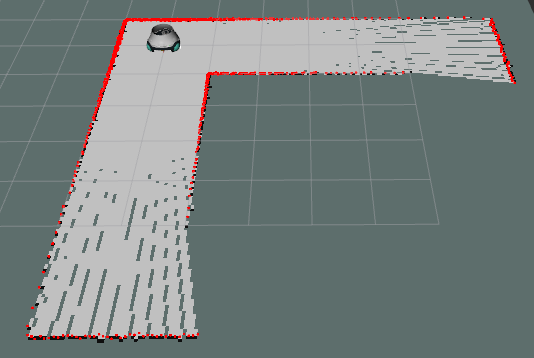
\includegraphics[width=.6\linewidth]{rviz_mapping}
    \caption{Running the automated parser node with Gmapping.}
    \label{fig:rviz_mapping}
\end{figure}

\section{Parsing the data}

The data parser is a Python node that will calculate the required metrics. It runs alongside the SLAM algorithm and constantly imports its information listening to the topics and computer resource information. When shut down, the node outputs the desired graphs and metrics. It can be called using the command:

\begin{verbatim}
rosrun cob_bringup_sim pipeline.py
\end{verbatim}

The node keeps executing the following tasks in parallel:

\begin{itemize}
    \item Republishes the ground truth from the ground truth topic (\texttt{/base\_pose\_ground\_truth}, as described in \prettyref{sec:collecting_data}) and republishes it as a tf, since it's easier to do transformations on. 
    \item Reads the \texttt{/tf} topic and stores a new pose into a pose history whenever the SLAM pose is updated, as well as the ground truth pose at that point in time.
    \item Collects data from CPU Usage and Memory Usage with an interval of 0.1 seconds.
\end{itemize}

When the node is shut down, the following tasks are executed:

\begin{itemize}
    \item The pose history is plotted alongside the ground truth.
    \item The squared pose error is calculated according to \prettyref{eq:error_squared}.
    \item The displacement pose error is calculated according to \prettyref{eq:displacement}.
    \item The CPU and Memory usage are plotted over time, using \texttt{psutil} library \cite{psutil}.
    \item The summary is generated including the average CPU usage, average Memory usage, translation displacement error, rotation displacement error, translation squared error, rotational squared error.
\end{itemize}

\section{Exporting the map}

The map can be exported using the the \texttt{map\_saver} node from the package \texttt{map\_server}. To export the map, simply call the node with the option \texttt{-f} and the map name.

\begin{verbatim}
rosrun map_server map_saver -f map_name
\end{verbatim}

Since Cartographer uses a different approach for generating submaps, the data has to be saved as a \texttt{.pbstream} first to generate the full map. To generate the map, we first have to tell the node to finish the trajectory calling the \texttt{/finish\_trajectory} service. Then, we export the \texttt{.pbstream} file and use it to generate the map. The following sequence of commands represent this process:

\begin{verbatim}
rosservice call /finish_trajectory 0
rosservice call /write_state "filename: '${HOME}/file.pbstream'"
rosrun cartographer_ros cartographer_pbstream_to_ros_map 
       -pbstream_filename ${HOME}/file.pbstream
\end{verbatim}

Because the resulting image for the map doesn't always have the right dimensions (approximately the same as the ground truth map), we have to crop the empty gray areas before running the map comparisons. We also want to convert from \texttt{.pgm} saved automatically to \texttt{.png} that the algorithm expects. To do that, we simply call the conversion function from ImageMagick, using the \texttt{-trim} options to trim the gray borders. Why the image is rotated 90 degrees is explained in the next section.

\begin{verbatim}
convert -rotate 90 map_name.pgm -trim map_name.png
\end{verbatim}

\section{Results}

All the mapping was done in the same machine equipped with an Intel Core i5-4430@3.00 GHz and 8 GB DDR3 memory. All the CPU measurements reflect the usage of a single core, meaning that values higher than 100\% represent the usage of more than one core at a time. The memory measurements are USS or "Unique Set Size", which is the amount of memory that would be freed if the process was terminated. The Gmapping version used was 1.3.10 \cite{gmappinggit}, the Hector version used was 0.3.5 \cite{hectorgit}, the Karto version used was 0.7.3 \cite{kartogit} and the Cartographer version used was 0.3.0 \cite{cartographergit}.

The mapping results for the three test maps designed on \prettyref{sec:selecting_maps} can be seen on \prettyref{fig:results1}, for the test map 1, \prettyref{fig:results2}, for the test map 2 and \prettyref{fig:results3} for the test map 3. The respective data collected during execution can be seen on \prettyref{tab:results1}, \prettyref{tab:results2} and \prettyref{tab:results3}.

At visual inspection, we can see that for the first map (\prettyref{fig:results1}), Karto Slam and Cartographer perform better, as the noise in the walls is lower. They look straight and sharp, as opposed to Gmapping and Hector, where the walls look noisy. If we inspect the results of \prettyref{tab:results1}, we can see that this reflects in Karto having the lowest localization error between all algorithms for this map for all metrics. Even though the Hector reconstruction is not as great, it scores second place in localization error, followed by Cartographer and finally Gmapping, although Cartographer is better at poses and Gmapping is better at angles.

In the second map, \prettyref{fig:results2}, the results are quite the opposite, with Hector and Cartographer performing better visually. Hector shows the best pose estimate in displacement, but Gmapping overcomes in squared error. Karto remains with good results but Cartographer lags behind. We can actually see why looking at the map, as Cartographer's map is tilted relative to the others. This error of orientation at the start was probably what made Cartographer perform worse in the localization.

In terms of average CPU and Memory usage, the values remained constant throughout the tests. Gmapping shows the highest usage of CPU among all algorithms, consuming almost double of Cartographer, in second place. Karto and Hector show low consumption of CPU, with Hector being the lowest. In terms of memory, Hector jumps ahead in all tests, followed by Gmapping, Hector and finally Cartographer. It is important to notice that despite having low CPU and memory footprint, we are only taking into consideration the SLAM node for Cartographer, and not the obstacle grid node nor the offline tasks executed by the \texttt{.pbstream} conversion.

\newpage
\begin{figure}[!ht]
     \centering
     \subfloat[][Gmapping]{\includegraphics[width=.4\linewidth]{gmapping/test1}\label{subfig:gmapping_test1}}
     \hspace{1cm}
     \subfloat[][Hector]{\includegraphics[width=.4\linewidth]{hector/test1}\label{subfig:hector_test1}}
     \\
     \subfloat[][Karto]{\includegraphics[width=.4\linewidth]{karto/test1}\label{subfig:karto_test1}}
     \hspace{1cm}
     \subfloat[][Cartographer]{\includegraphics[width=.4\linewidth]{cartographer/test1}\label{subfig:cartographer_test1}}
     \caption{Results of mapping for first map.}
     \label{fig:results1}
\end{figure}

\begin{table}[!ht]
\centering
\renewcommand*{\arraystretch}{1.1}
\begin{tabular}{c|c|c|c|c}
& \textbf{Gmapping} & \textbf{Hector} & \textbf{Karto} & \textbf{Cartographer} \\ \hline
\textbf{Pose displacement} & 0.0010116 & 0.00051379 & \textbf{0.00014934} & 0.00095104 \\
\textbf{Angle displacement} & 4.0385e-05 & 2.3272e-05 & \textbf{1.2402e-05} & 0.00010114 \\
\textbf{Pose squared error} & 0.0018224 & 0.00058361 & \textbf{0.00024294} & 0.00086193 \\
\textbf{Angle squared error} & 2.0899e-05 & 1.6251e-05 & \textbf{6.9566e-06} & 6.3385e-05 \\
\textbf{CPU (\%)} & 14.36 & \textbf{3.67} & 4.74 & 7.13 \\
\textbf{Memory (MB)} & 19.56 & 26.39 & 13.18 & \textbf{12.52} \\ \hline
\end{tabular}
\caption{Data collected for the first map (lower is better).}
\label{tab:results1}
\end{table}


\begin{figure}[!ht]
     \centering
     \subfloat[][Gmapping]{\includegraphics[width=.4\linewidth]{gmapping/test2}\label{subfig:gmapping_test2}}
     \hspace{1cm}
     \subfloat[][Hector]{\includegraphics[width=.4\linewidth]{hector/test2}\label{subfig:hector_test2}}
     \\
     \subfloat[][Karto]{\includegraphics[width=.4\linewidth]{karto/test2}\label{subfig:karto_test2}}
     \hspace{1cm}
     \subfloat[][Cartographer]{\includegraphics[width=.4\linewidth]{cartographer/test2}\label{subfig:cartographer_test2}}
     \caption{Results of mapping for second map.}
     \label{fig:results2}
\end{figure}

\begin{table}[!ht]
\centering
\renewcommand*{\arraystretch}{1.1}
\begin{tabular}{c|c|c|c|c}
& \textbf{Gmapping} & \textbf{Hector} & \textbf{Karto} & \textbf{Cartographer} \\ \hline
\textbf{Pose displacement} & 0.00037009 & \textbf{0.00024439} & 0.0031410 & 0.013768 \\
\textbf{Angle displacement} & 3.6161e-05 & 2.6309e-05 & \textbf{1.0607e-05} & 4.4936e-05 \\
\textbf{Pose squared error} & \textbf{0.00038672} & 0.0010135 & 0.0035834 & 0.013529 \\
\textbf{Angle squared error} & 0.00038672 & \textbf{2.5932e-05} & 0.00016662 & 0.00060306 \\
\textbf{CPU (\%)} & 11.38 & \textbf{3.75} & 4.72 & 6.56 \\
\textbf{Memory (MB)} & 19.11 & 26.50 & 14.45 & \textbf{12.33} \\ \hline
\end{tabular}
\caption{Data collected for the second map (lower is better).}
\label{tab:results2}
\end{table}

\begin{figure}[!ht]
     \centering
     \subfloat[][Gmapping]{\includegraphics[width=.4\linewidth]{gmapping/test3}\label{subfig:gmapping_test3}}
     \hspace{1cm}
     \subfloat[][Hector]{\includegraphics[width=.4\linewidth]{hector/test3}\label{subfig:hector_test3}}
     \\
     \subfloat[][Karto]{\includegraphics[width=.4\linewidth]{karto/test3}\label{subfig:karto_test3}}
     \hspace{1cm}
     \subfloat[][Cartographer]{\includegraphics[width=.4\linewidth]{cartographer/test3}\label{subfig:cartographer_test3}}
     \caption{Results of mapping for third map.}
     \label{fig:results3}
\end{figure}

\begin{table}[!ht]
\centering
\renewcommand*{\arraystretch}{1.1}
\begin{tabular}{c|c|c|c|c}
& \textbf{Gmapping} & \textbf{Hector} & \textbf{Karto} & \textbf{Cartographer} \\ \hline
\textbf{Pose displacement} & 0.015545 & 0.013457 & 0.0050207 & \textbf{0.0012753} \\
\textbf{Angle displacement} & 6.0892e-05 & 9.0999e-05 & 5.0616e-05 & \textbf{4.7758e-05} \\
\textbf{Pose squared error} & 0.022001 & 0.015299 & 0.0054754 & \textbf{0.0026521} \\
\textbf{Angle squared error} & 0.00055478 & 0.00080006 & 0.00033509 & \textbf{2.8089e-05} \\
\textbf{CPU (\%)} & 12.04 & \textbf{3.73} & 4.99 & 6.30 \\
\textbf{Memory (MB)} & 19.88 & 26.32 & 15.88 & \textbf{14.45} \\ \hline
\end{tabular}
\caption{Data collected for the third map (lower is better).}
\label{tab:results3}
\end{table}
\clearpage

In the third map, Cartographer seems to outperform every other algorithm in every metric, resulting in a much better map, followed by Karto, and finally Gmapping and Hector with very similar results. It is clear from analyzing the pose error from all the algorithm runs that this method is not giving a good way of measuring accuracy, at least for this test case.

The results of running the ICP matcher with the algorithms can be seen on \prettyref{tab:results_icp}. The best algorithm in all cases was Cartographer, scoring lowest. This means two things: most of the walls were placed in the correct spot and the noise is low. In the second place, Gmapping could outperform Hector and Karto, justifying the wide adoption of Gmapping in the robotic world, as it is far easier to set up than Cartographer. Hector and Karto were tied in the last position in this test, as Hector was better at the first map, Karto was better in the second map and the results are approximately the same in the third map.

\begin{table}[!ht]
\centering
\renewcommand*{\arraystretch}{1.1}
\begin{tabular}{c|c|c|c|c}
& \textbf{Gmapping} & \textbf{Hector} & \textbf{Karto} & \textbf{Cartographer} \\ \hline
\textbf{Test 1} & 0.46144 & 0.61088 & 0.75229 & \textbf{0.34752} \\
\textbf{Test 2} & 0.55829 & 0.76593 & 0.62868 & \textbf{0.51959} \\
\textbf{Test 3} & 0.64751 & 0.78693 & 0.75315 & \textbf{0.41721} \\
 \hline
\end{tabular}
\caption{Results of running ICP over maps (lower is better).}
\label{tab:results_icp}
\end{table}

When modeling free space, most of the algorithms show the same result, with Gmapping showing slightly better results than the other. One of the problems Gmapping faces, though, is mapping places inside the walls where it has no information about, as shown on \prettyref{fig:gmapping_error}. This results in more free space being shown than normal, which might indicate why Gmapping has a lower score. All the algorithms have results with a positive sign, meaning that the less free space was mapped than in fact exists, which is good, as discussed in \prettyref{sec:free_space}.

\begin{figure}[!ht]
     \centering
     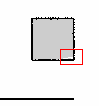
\includegraphics[width=.4\linewidth]{gmapping_error}
     \caption{Incorrect mapping from Gmapping on test 2.}
     \label{fig:gmapping_error}
\end{figure}

\begin{table}[!ht]
\centering
\renewcommand*{\arraystretch}{1.1}
\begin{tabular}{c|c|c|c|c}
& \textbf{Gmapping} & \textbf{Hector} & \textbf{Karto} & \textbf{Cartographer} \\ \hline
\textbf{Test 1 (\%)} & \textbf{3.71} & 4.15 & 4.98 & 4.91 \\
\textbf{Test 2 (\%)} & \textbf{3.68} & 4.80 & 4.61 & 6.09 \\
\textbf{Test 3 (\%)} & \textbf{3.90} & 5.24 & 5.02 & 5.79 \\
 \hline
\end{tabular}
\caption{Results of free space mapping accuracy (lower is better).}
\label{tab:results_whitespace}
\end{table}

We are going to analyze the CPU and Memory profiles for each algorithm running in the second map. Figures \ref{fig:gmapping_cpu} to \ref{fig:cartographer_cpu} show both the CPU usage and RAM Memory used over time. The $x$ axis represents the number of samples, and since the acquisition frequency was 10 Hz, every 500 samples are equivalent to 50 seconds.

\prettyref{fig:gmapping_cpu} shows how Gmapping performs when running. It is possible to see that the CPU peaks at a value of more than 100\% every few iterations, and most of the time it stays around 10\%. This peak every few iterations is the result of each laser scan being processed, and the effort seems to stay constant until the end, peaking around the same value. The memory grows in small incremental steps as the map is being constructed, and stops at around 1000 samples, where the map is already near the final state and only a few bits of new information are added.

\begin{figure}[!ht]
    \centering
    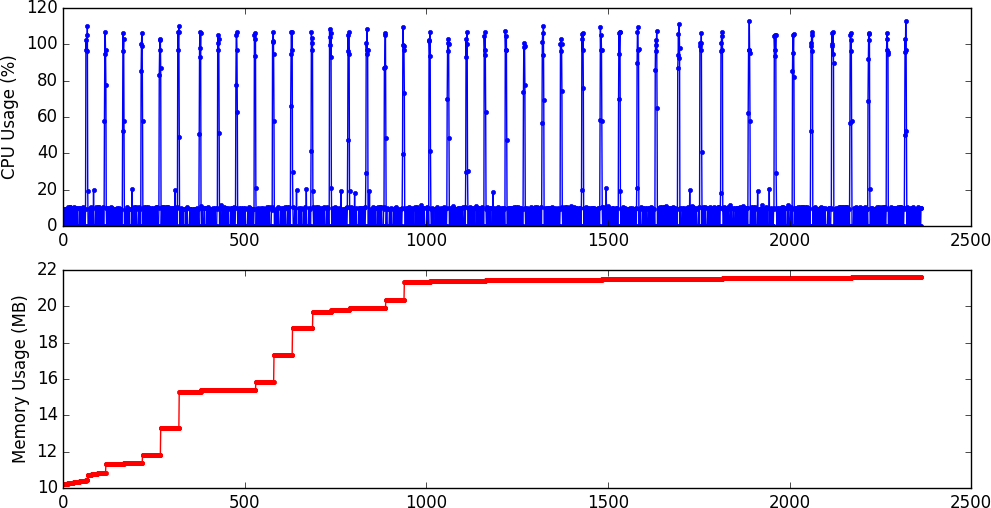
\includegraphics[width=.8\linewidth]{gmapping_cpu}
    \caption{CPU and Memory usage for Gmapping running map test 2.}
    \label{fig:gmapping_cpu}
\end{figure}

As already mentioned, Hector performs better on CPU and worse on memory. \prettyref{fig:hector_cpu} shows peaks around 20 \% and around 10 \%. Most of the time, the algorithm stays idle, to account for the average CPU usage of around 4 \%. Memory consumption, in this case, is high from the start and stays the same until the end. One of the reasons might be because it allocates the whole map right from the start, instead of allocating memory for a small map and increasing as new areas are discovered.

\begin{figure}[!ht]
    \centering
    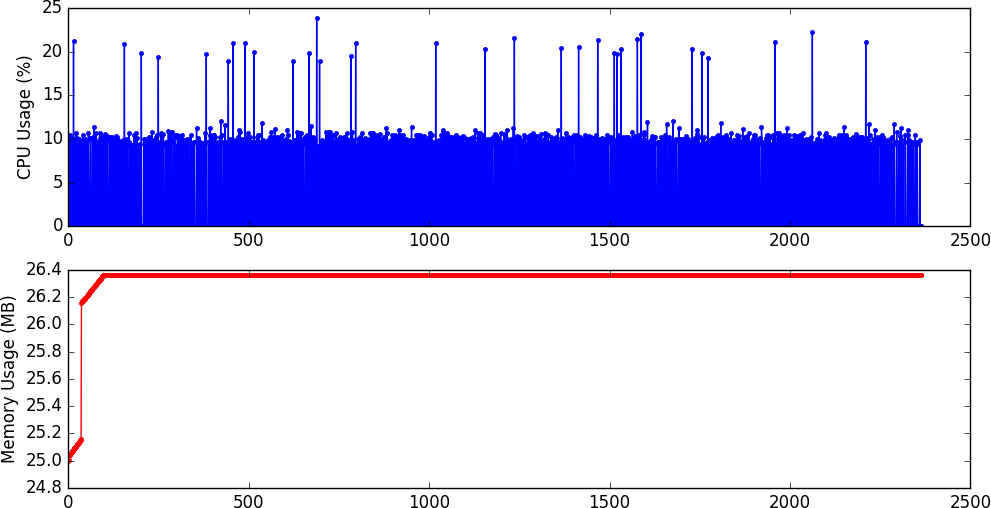
\includegraphics[width=.8\linewidth]{hector_cpu}
    \caption{CPU and Memory usage for Hector running map test 2.}
    \label{fig:hector_cpu}
\end{figure}

The results for Karto can be seen on \prettyref{fig:karto_cpu}. For CPU, we can see that the peaks become higher as the algorithm is executed for longer. This is expected as the problem of optimizing a pose-graph becomes harder as more nodes are added to the graph. The memory seems to grow linearly as time progresses, even though no more information is being added after some point in time.

\begin{figure}[!ht]
    \centering
    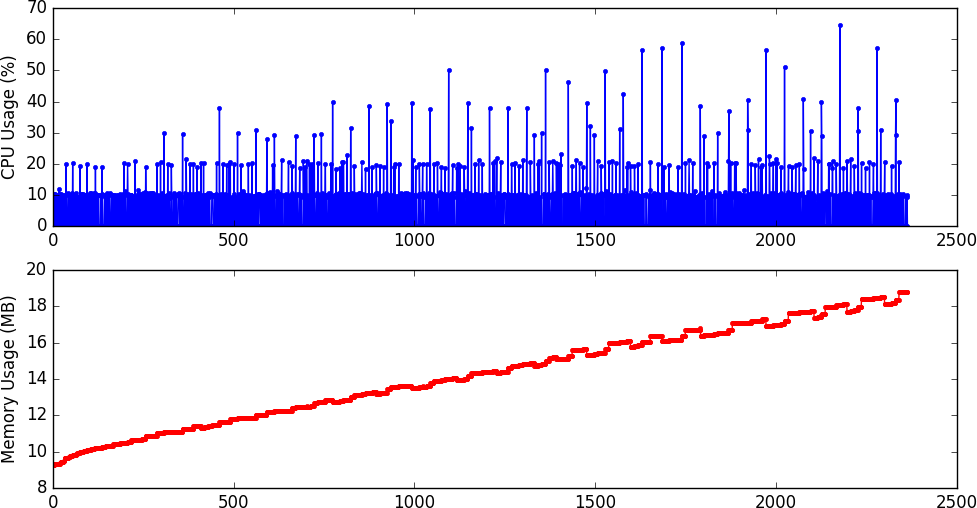
\includegraphics[width=.8\linewidth]{karto_cpu}
    \caption{CPU and Memory usage for Karto running map test 2.}
    \label{fig:karto_cpu}
\end{figure}

Finally, the results for Cartographer can be seen on \prettyref{fig:cartographer_cpu}. It behaves similar to Gmapping, although with lower peaks, with the memory growing linearly like Karto, with small bumps every 1000 samples.

\begin{figure}[!ht]
    \centering
    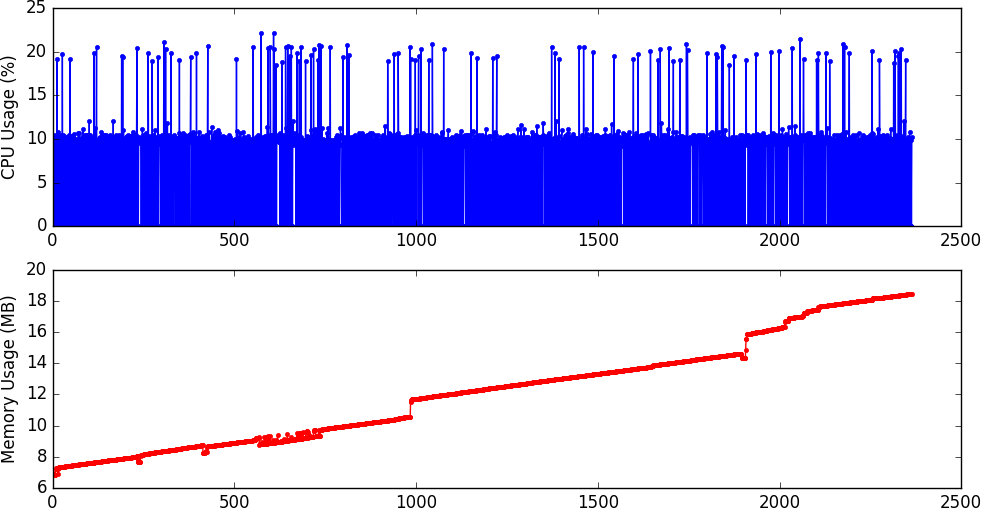
\includegraphics[width=.8\linewidth]{cartographer_cpu}
    \caption{CPU and Memory usage for Cartographer running map test 2.}
    \label{fig:cartographer_cpu}
\end{figure}

In terms of results, the temporal analysis of the graphs brings additional information to the table. All the algorithms show consumption around 10\%, differentiating on the peaks and the amount they stay idle. Gmapping was the most intensive on CPU, especially because of all the peaks. Hector and Karto stayed with low consumption and Cartographer were very modest considering its complexity. 